\documentclass{beamer}

\usepackage[utf8]{inputenc}
\usepackage{default}
\usepackage{amsfonts,amsmath,amssymb,amsthm,amstext,latexsym}
\usepackage{listings}
\usepackage{tikz}
\usetikzlibrary{calc}
\usetikzlibrary{arrows,shapes}
\usetikzlibrary{patterns,snakes}
\definecolor{mygray}{gray}{0.9}

\begin{document}

\begin{frame}

  \begin{center}
    \Huge
    Approximate computing
  \end{center}
  Reduce the execution time of an application by giving inexact results.
  \pause
  \begin{itemize}
    \item Precision of a floating-point value
    \item No exact result exists (search query...)
    \item ...
  \end{itemize}
  \pause
  \begin{itemize}
   \item Skip steps in loops
   \item Branching to avoid useless computations
   \item Faulty hardware (fast adders...)
   \item ...
  \end{itemize}

\end{frame}

\begin{frame}{Multi-grid}
 Solve $\beta u''(x)+\alpha u(x)=f(x)$ in $u$, on $[0;1]$ and $u(0)=u(1)=0$.\\ \vspace{0.3cm}
 Interpolate function on a grid of step $h=\frac{1}{N}$, $x_i = \frac{i}{N}$, $i=0..N$.\\
 $u''(x_i) \approx \frac{u(x_{i-1})-2u(x_i)+u(x_{i+1})}{h^2} \Rightarrow Au = f$, $A \in \mathcal{M}_n(\mathbb{R}^{N-1xN-1})$.\\ \vspace{0.3cm}
 
 Then relax, $u_{i+1} = M u_{i} + N f$. What is $u_{0}$? How fast does it converge to $u$?
\end{frame}

\begin{frame}{Multi-grid}
 The idea is to use different values of $h$, different grids: $h,2h,\dots,H$.\\
 $u^{2h}$ can be a good initial guess for $u^h_0$.\\
 It also improves the convergence speed.\vspace{0.5cm}
 
 Two measures have to be taken into account, the error $e$ and the residual $r$: $u = u_i + e_i \Rightarrow Ae_i = f-Au_i = r_i$.
 
\end{frame}

\begin{frame}{Multi-grid}
  V-cycle$(h,H,\alpha_1,\alpha_2)$:\\
  \begin{enumerate}
    \item $s \leftarrow h; u^h\leftarrow0$
   \item Relax $\alpha_1$ times on grid $s$, initial guess $u^s$.
   \item if $s<H$ : $f^{2s} \leftarrow I_{s\rightarrow 2s}(f^s-A^su^s)$,$u^{2s}\leftarrow0$,$s \leftarrow 2s$ and goto 2.
   \item $u^s \leftarrow u^s+I_{2s\rightarrow s} u^{2s}$.
   \item Relax $\alpha_2$ times on grid $s$, initial guess $u^s$
   \item if $s > h$ : $s = s/2$ and goto 4.
  \end{enumerate}

  Two ways of controlling the execution time and precision: limiting the number of steps ($\alpha_1,\alpha_2$), do several V-cycles and stopping when reaching a given precision $\epsilon$ or a maximum number of V-cycles.
  
\end{frame}

\begin{frame}{BoomerAMG and AMG2006}
  
  \begin{itemize}
   \item Execute 3D problems (Laplace on a cube...)
   \item Default parameters: 8x8x8=512 variables
   \item Solved with preconditioned conjudate gradient, using BoomerAMG preconditioner (HYPRE library)
   \pause
   \item Measures done on execution of BoomerAMG algorithm to directly solve $Ax=b$, not as preconditioner!
   \item Different parameters to play with:
    \begin{itemize}
      \item Tolerance ($\epsilon$) for relative residual norm
      \item Max number of cycles
      \item Type of cycle
      \item Number of relaxations at each step
      \item Number of variables
    \end{itemize}
    
  \end{itemize}
 
\end{frame}

\begin{frame}{Types of cycle}
 \begin{figure}
 %\resizebox{\linewidth}{4cm}{
 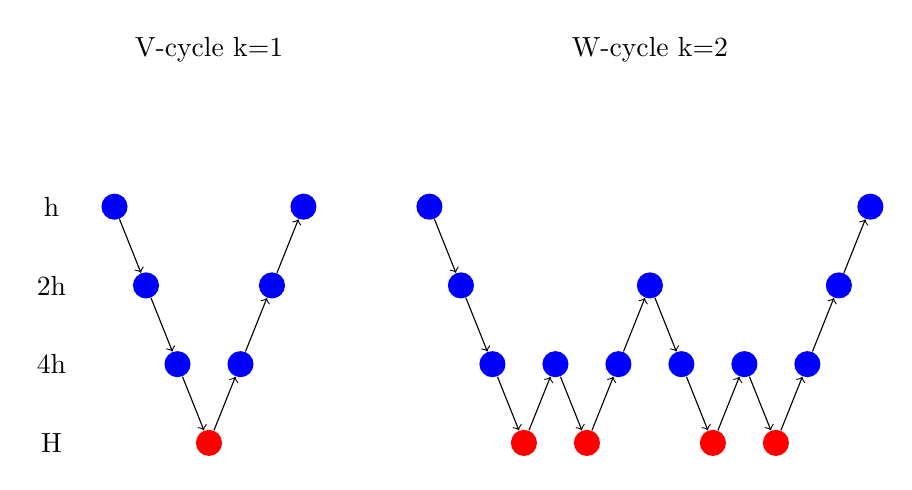
\begin{tikzpicture}
 
 
\begin{scope}[xscale=2/5]

  \node (sh) at (-5,3) { h };
  \node (shh) at (-5,2) { 2h };
  \node (shhh) at (-5,1) { 4h };
  \node (shhhh) at (-5,0) { H };
  
  \node (title) at (0,5) { V-cycle k=1};
  \node (title2) at (14,5) {W-cycle k=2};

    \node[circle,fill=blue] (a) at (-3,3) { };
    \node[circle,fill=blue] (b) at (-2,2) {};
    \node[circle,fill=blue] (c) at (-1,1) {};
    \node[circle,fill=red] (d) at (0,0) {};
    \node[circle,fill=blue] (e) at (1,1) {};
    \node[circle,fill=blue] (f) at (2,2) {};
    \node[circle,fill=blue] (g) at (3,3) {};
    
    \draw[->] (a) -- (b);
    \draw[->] (b) -- (c);
    \draw[->] (c) -- (d);
    \draw[->] (d) -- (e);
    \draw[->] (e) -- (f);
    \draw[->] (f) -- (g);
    
    \node[circle,fill=blue] (aa) at (7,3) { };
    \node[circle,fill=blue] (ab) at (8,2) {};
    \node[circle,fill=blue] (ac) at (9,1) {};
    \node[circle,fill=red] (ad) at (10,0) {};
    \node[circle,fill=blue] (ae) at (11,1) {};
    \node[circle,fill=red] (af) at (12,0) {};
    \node[circle,fill=blue] (ag) at (13,1) {};
    \node[circle,fill=blue] (ah) at (14,2) {};
    \node[circle,fill=blue] (ai) at (15,1) {};
    \node[circle,fill=red] (aj) at (16,0) {};
    \node[circle,fill=blue] (ak) at (17,1) {};
    \node[circle,fill=red] (al) at (18,0) {};
    \node[circle,fill=blue] (am) at (19,1) {};
    \node[circle,fill=blue] (an) at (20,2) {};
    \node[circle,fill=blue] (ao) at (21,3) {};
    
    \draw[->] (aa) -- (ab);
    \draw[->] (ab) -- (ac);
    \draw[->] (ac) -- (ad);
    \draw[->] (ad) -- (ae);
    \draw[->] (ae) -- (af);
    \draw[->] (af) -- (ag);
    \draw[->] (ag) -- (ah);
    \draw[->] (ah) -- (ai);
    \draw[->] (ai) -- (aj);
    \draw[->] (aj) -- (ak);
    \draw[->] (ak) -- (al);
    \draw[->] (al) -- (am);
    \draw[->] (am) -- (an);
    \draw[->] (an) -- (ao);
    \end{scope}
    
 \end{tikzpicture}
 %}
\end{figure}
 
\end{frame}

\begin{frame}{Cost of a $k$-cycle}
 
 Using a grid with $N$ points for each of the $d$ dimensions, doing $s$ relaxations at each level:
 \begin{itemize}
  \item V-cycle (1-cycle) costs $\leq \frac{2}{1-2^{-d}} sN^d$
  \item W-cycle (2-cycle) costs $\leq \frac{3}{1-2^{1-d}} sN^d$
  \item $k$-cycle costs $\leq \frac{k+1}{1-k2^{-d}} sN^d$
  \end{itemize}
\end{frame}

\begin{frame}{Results - 80x80x80}
 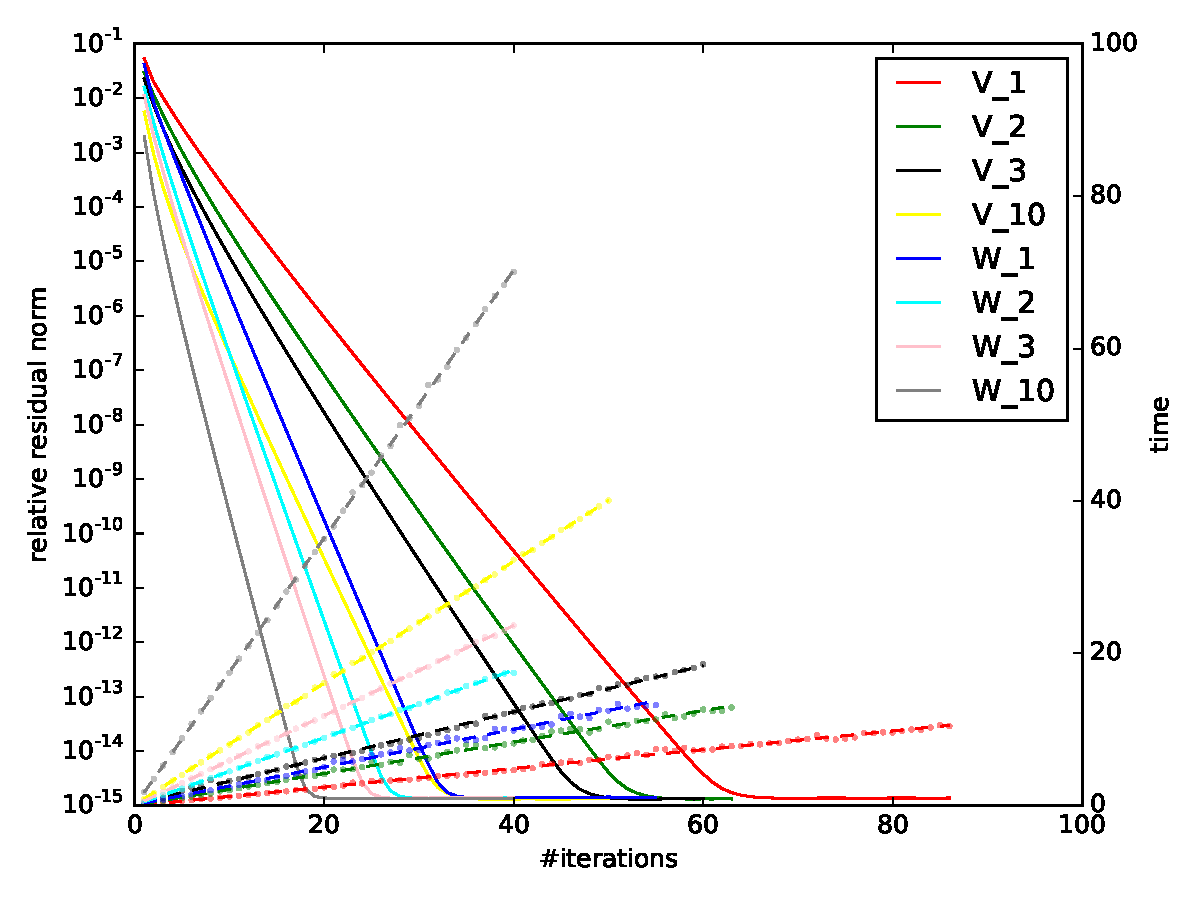
\includegraphics[width=\linewidth]{AMG2006/test/edit/convergence_1.pdf}
\end{frame}
\begin{frame}{Results - 80x80x80}
 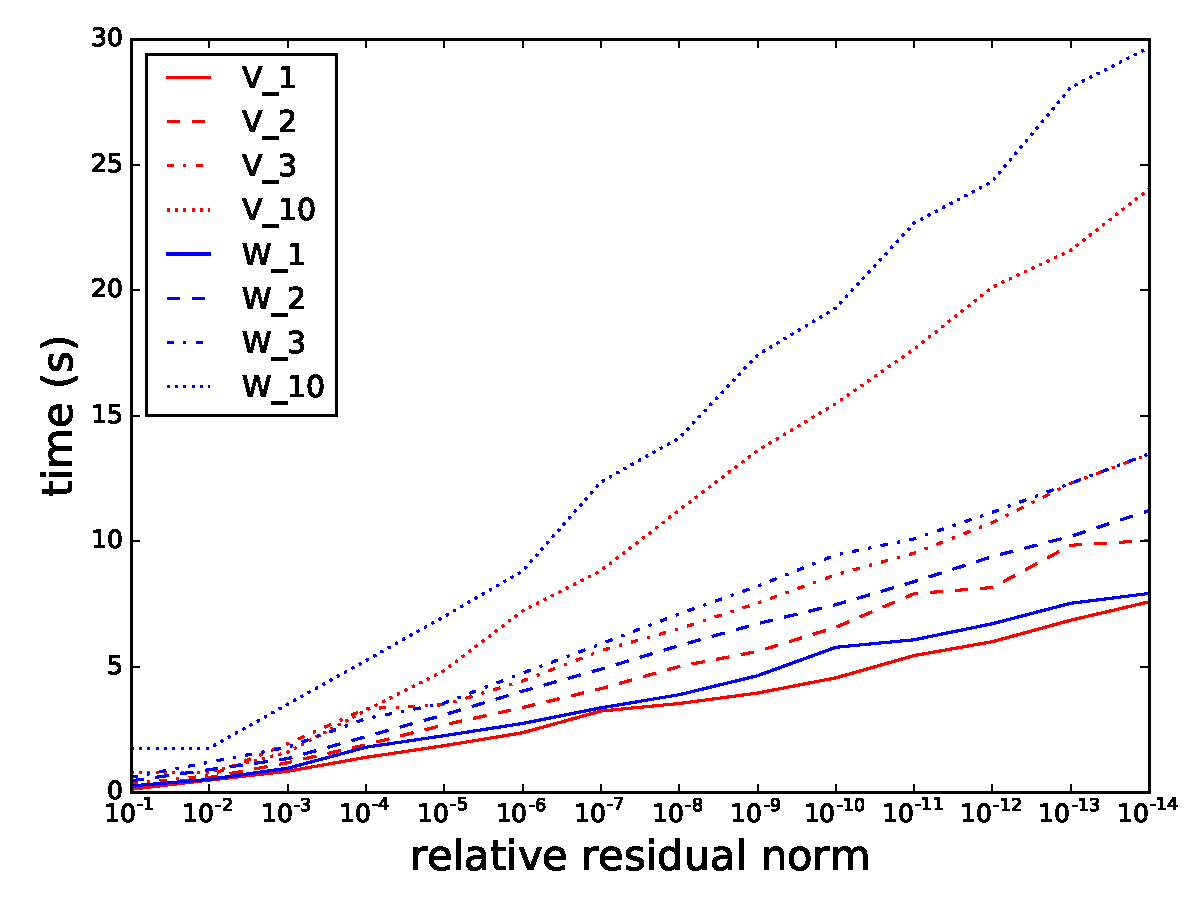
\includegraphics[width=\linewidth]{AMG2006/test/edit/time_convergence.pdf}
\end{frame}
\begin{frame}{Results - 40x40x40}
 \includegraphics[width=\linewidth]{AMG2006/test/edit/convergence_1_small.pdf}
\end{frame}
\begin{frame}{Results - 40x40x40}
 \includegraphics[width=\linewidth]{AMG2006/test/edit/time_convergence_small.pdf}
\end{frame}

\begin{frame}{Results}
80x80x80:
\vspace{-0.8cm}
 \begin{table}
  \resizebox{\linewidth}{!}{
     \begin{tabular}{|c||c|c|c|c||c|c|c|c|}
     \hline
       Parameters & V (1) & V (2) & V (3) & V (10) & W (1) & W (2) & W (3) & W (10) \\
     \hline
       Slope	  & 0.123 & 0.207 & 0.304 & 0.799 & 0.248 & 0.443 & 0.591 & 1.758 \\
     \hline
       Offset     & -0.046 & 0.069 & 0.151 & 0.082 & 0.078 & 0.038 & -0.003 & -0.030 \\
     \hline
     \end{tabular}
  }
 \end{table}
\vspace{-0.5cm}
 \begin{table}
     \begin{tabular}{|c|c|c|c|c|c|}
     \hline
       W/V & 1 & 2 & 3 & 10 & Theoretical \\
     \hline
       Value	  & 2.018 & 2.149 & 1.947 & 2.199 & 1.75 \\
     \hline
     \end{tabular}
 \end{table}

40x40x40:
\vspace{-0.8cm}
 \begin{table}
  \resizebox{\linewidth}{!}{
     \begin{tabular}{|c||c|c|c|c||c|c|c|c|}
     \hline
       Parameters & V (1) & V (2) & V (3) & V (10) & W (1) & W (2) & W (3) & W (10) \\
     \hline
       Slope	  & 0.0188 & 0.0298 & 0.0379 & 0.115 & 0.0317 & 0.0547 & 0.0722 & 0.214 \\
     \hline
       Offset     & -0.0340 & -0.0801 & 0.0279 & 0.0382 & 0.00229 & -0.0768 & -0.0397 & -0.0312 \\
     \hline
     \end{tabular}
  }
 \end{table}
\vspace{-0.5cm}
 
 \begin{table}
     \begin{tabular}{|c|c|c|c|c|c|}
     \hline
       W/V & 1 & 2 & 3 & 10 & Theoretical \\
     \hline
       Value	  & 1.685 & 1.836 & 1.906 & 1.852 & 1.75 \\
     \hline
     \end{tabular}
 \end{table}
 
 Ratio between 10x10x10 and 5x5x5 is between 6.540 and 8.561 (average 7.644).
 
 
\end{frame}

\begin{frame}{Execution times in a V-cycle}
 Problem size: 80x80x80. Grid levels: 8.\\ \vspace{0.5cm}
 \resizebox{\linewidth}{!}{
 \begin{tabular}{|c|c|c|c|c|c|c|}
 \hline
 Level & Matrix size & Non-zero & Relax (down) & Relax (up) & Matvec (down) & Matvec (up) \\
 \hline
  0 & 512,000 & 4,042,520 & 20 ms & 20 ms & 15 ms & -\\
 \hline
  1 & 256,000 & 6,475,239 & 20 ms & 25 ms & 12 ms & 4 ms\\
 \hline
  2 & 58893 & 2,000,513 & 8 ms & 8 ms & 3 ms & 2 ms\\
 \hline
  3 & 14285 & 788,509 & 2 ms & 2 ms & 1 ms & 0.7 ms\\
 \hline
  4 & 4238 & 386,333 & 1 ms & 1 ms & 0.5 ms & 0.2 ms\\
 \hline
  5 & 609 & 53,493 & 0 ms & 0 ms & 0 ms & 0 ms\\
 \hline
  6 & 69 & 2,873 & 0 ms & 0 ms & 0 ms & 0 ms\\
 \hline
  7 & 2 & 4 & 0 ms & - & - & 0 ms\\
 \hline
 \end{tabular}
 }\\ \vspace{0.5cm}
Globally, relaxation represents $\approx$66\% of the time of a V-cycle, and matrix-vector products $\approx$25-30\%.
 \end{frame}

\begin{frame}{Ideas}
  Idea: remove or add relaxation steps at given levels $l \in 0,\dots,n-1$.\\
  Observations: removing relaxation steps at finer levels is \textbf{less efficient}. Adding relaxation steps at coarser levels is \textbf{useless}.
  Strategies tested:\\
  \begin{itemize}
   \item \emph{Fast} : no relaxation at level 1.
   \item \emph{Fast2} : 10 relaxations at level $n-3$.
   \item \emph{Fast3} : 2 relaxations at levels $n-3,n-5,\dots,2$.
   \item \emph{Fast4} : no relaxation at level 2.
  \end{itemize}
\end{frame}

\begin{frame}{Results - 40x40x40}
 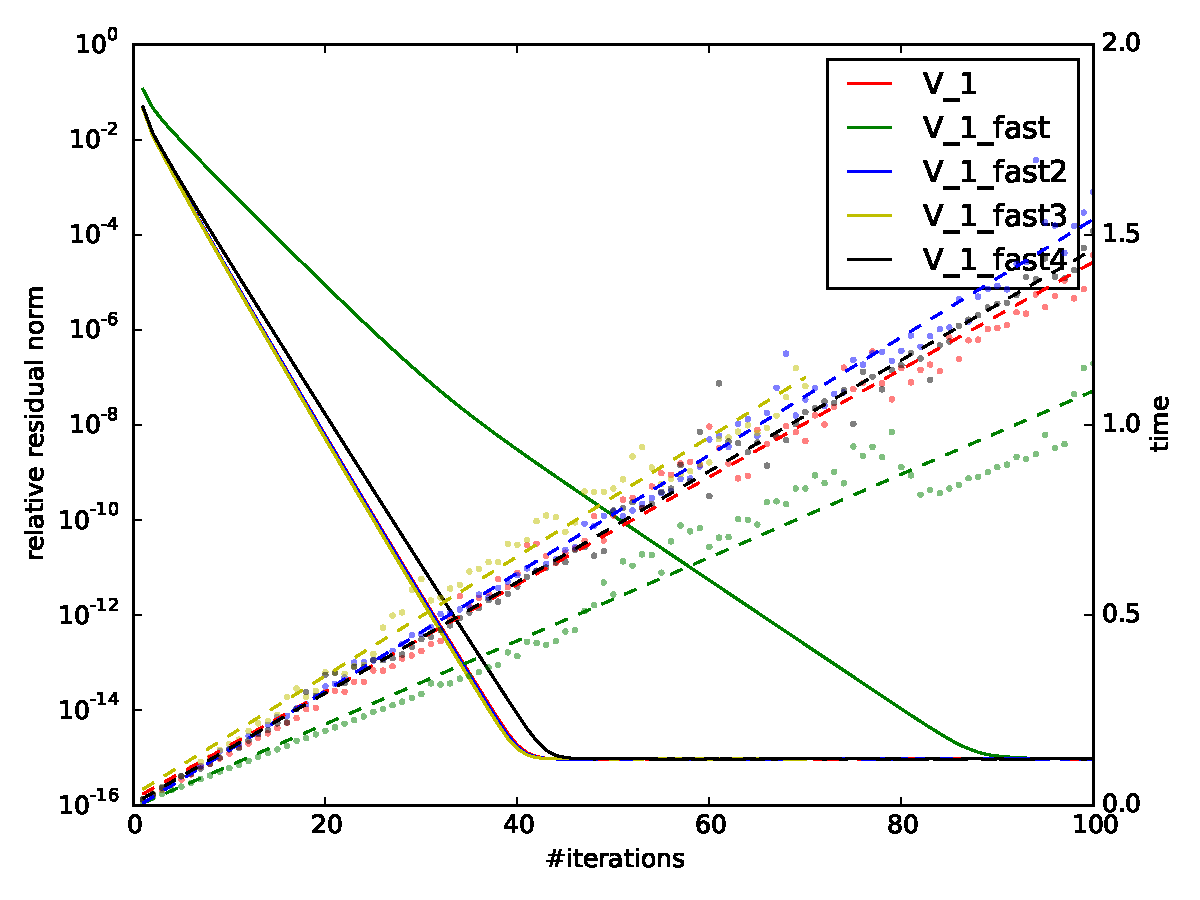
\includegraphics[width=\linewidth]{AMG2006/test/edit/convergence_fast_small.pdf}
\end{frame}
\begin{frame}{Results - 40x40x40}
 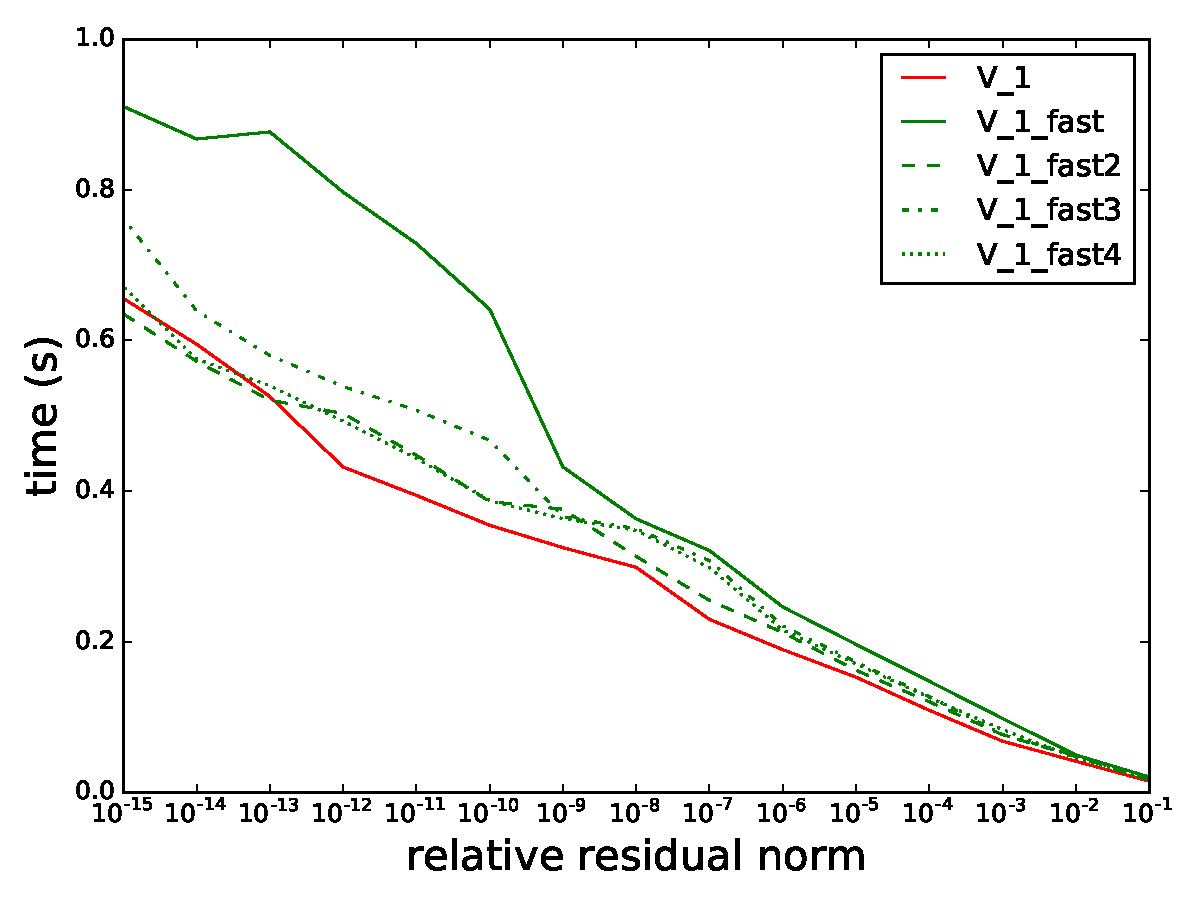
\includegraphics[width=\linewidth]{AMG2006/test/edit/time_convergence_fast_small.pdf}
\end{frame}
\begin{frame}{Results - 80x80x80}
 \includegraphics[width=\linewidth]{AMG2006/test/edit/convergence_fast.pdf}
\end{frame}
\begin{frame}{Results - 80x80x80}
 \includegraphics[width=\linewidth]{AMG2006/test/edit/time_convergence_fast.pdf}
\end{frame}

\begin{frame}{Ideas}
  Idea: remove or add relaxation steps at given levels $l \in 0,\dots,n-1$.\\
  Observations: removing relaxation steps at finer levels is \textbf{less efficient}. Adding relaxation steps at coarser levels is \textbf{useless}.
  Strategies tested:\\
  \begin{itemize}
   \item {\color{mygray}\emph{Fast} : no relaxation at level 1.
   \item \emph{Fast2} : 10 relaxations at level $n-3$.
   \item \emph{Fast3} : 2 relaxations at levels $n-3,n-5,\dots,2$.}
   \item \emph{Fast4} : no relaxation at level 2.
   \item \emph{Up} : relaxation only when going up in the cycle.
  \end{itemize}
\end{frame}
\begin{frame}{Results - 80x80x80}
 \includegraphics[width=\linewidth]{AMG2006/test/ASUS/convergence_fast.pdf}
\end{frame}
\begin{frame}{Results - 80x80x80}
 \includegraphics[width=\linewidth]{AMG2006/test/ASUS/time_convergence_fast.pdf}
\end{frame}
\begin{frame}{Results - 80x80x80 - Laplace27pt}
 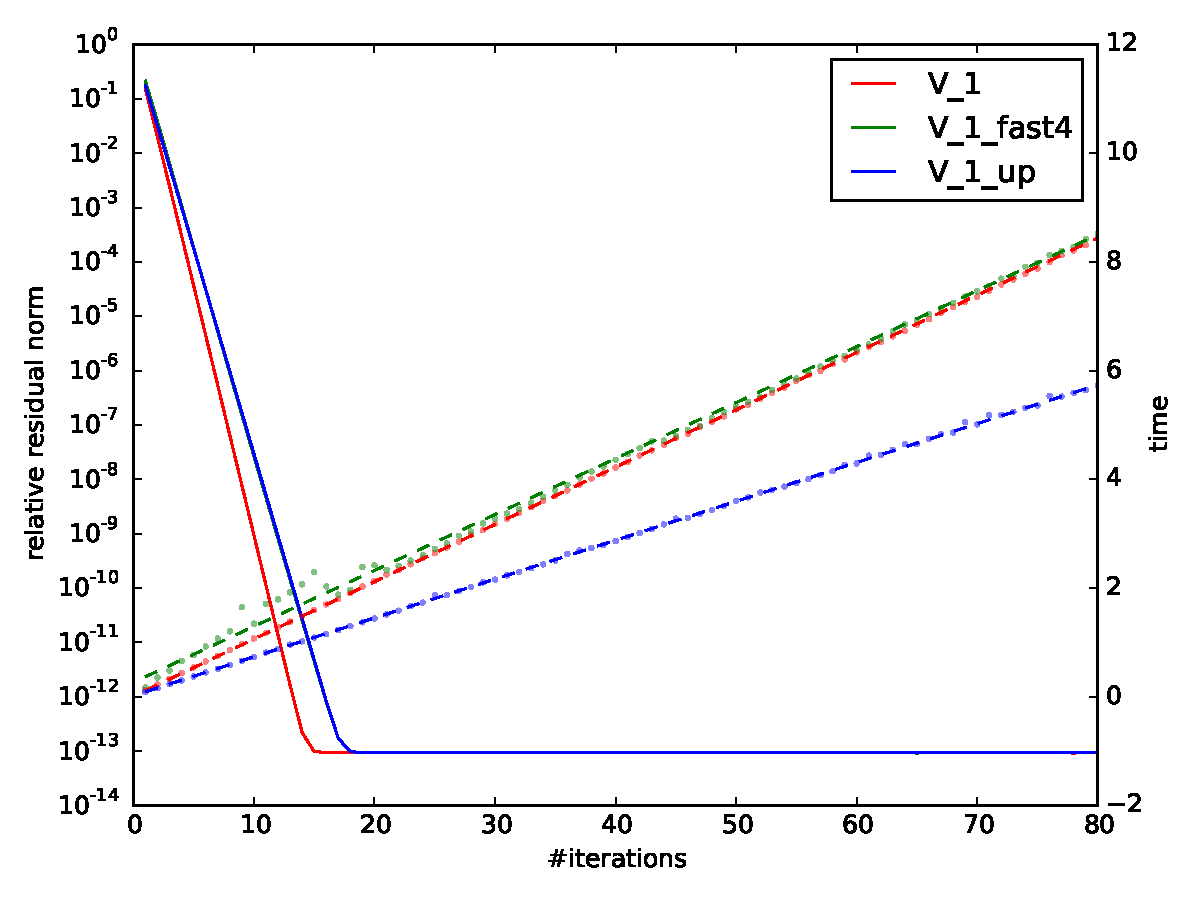
\includegraphics[width=\linewidth]{AMG2006/test/DELL/27pt/convergence_fast_10.pdf}
\end{frame}
\begin{frame}{Results - 80x80x80 - Laplace27pt}
 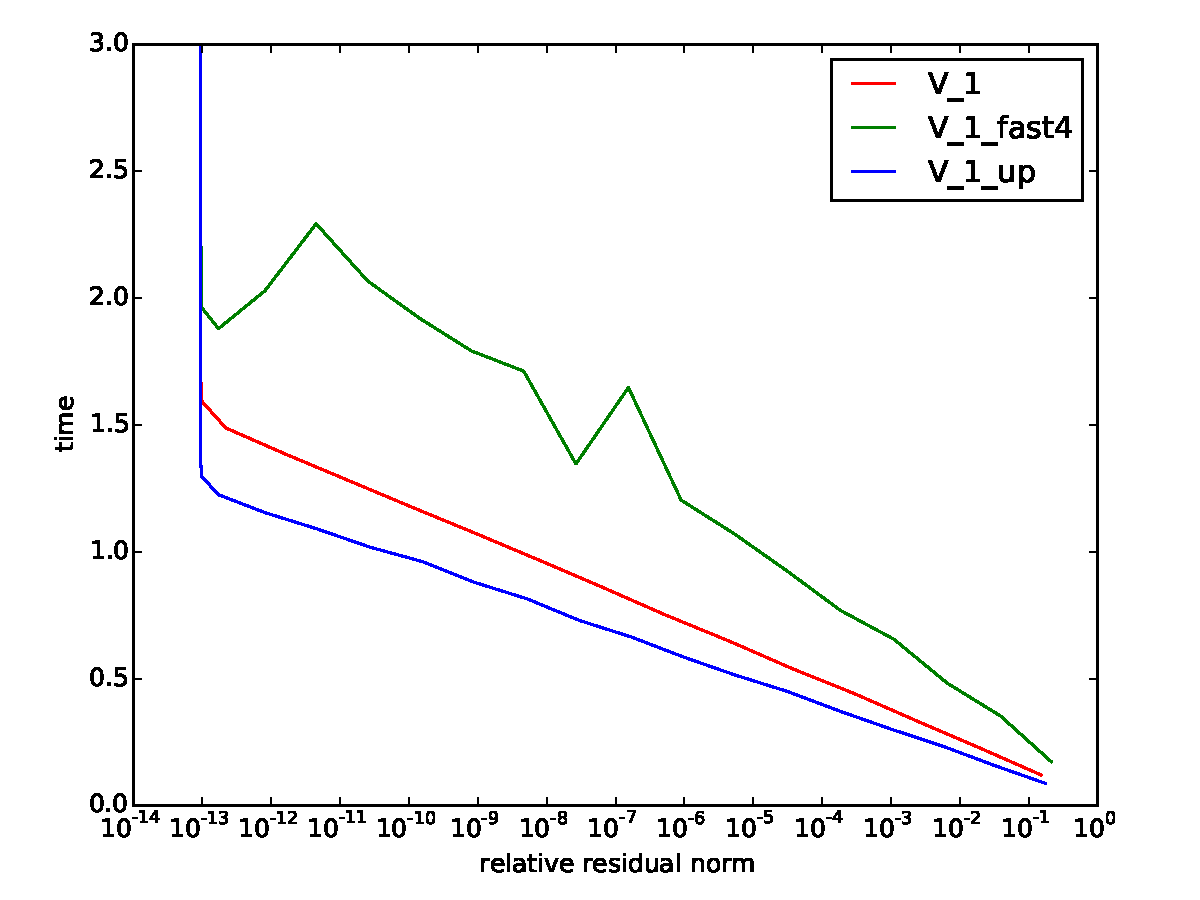
\includegraphics[width=\linewidth]{AMG2006/test/DELL/27pt/time_convergence_fast_10.pdf}
\end{frame}
\begin{frame}{Results - 40x40x40 - Laplace27pt}
 \includegraphics[width=\linewidth]{AMG2006/test/DELL/27pt/convergence_fast.pdf}
\end{frame}
\begin{frame}{Results - 40x40x40 - Laplace27pt}
 \includegraphics[width=\linewidth]{AMG2006/test/DELL/27pt/time_convergence_fast.pdf}
\end{frame}
\begin{frame}{Results - 80x80x80 - Laplace}
 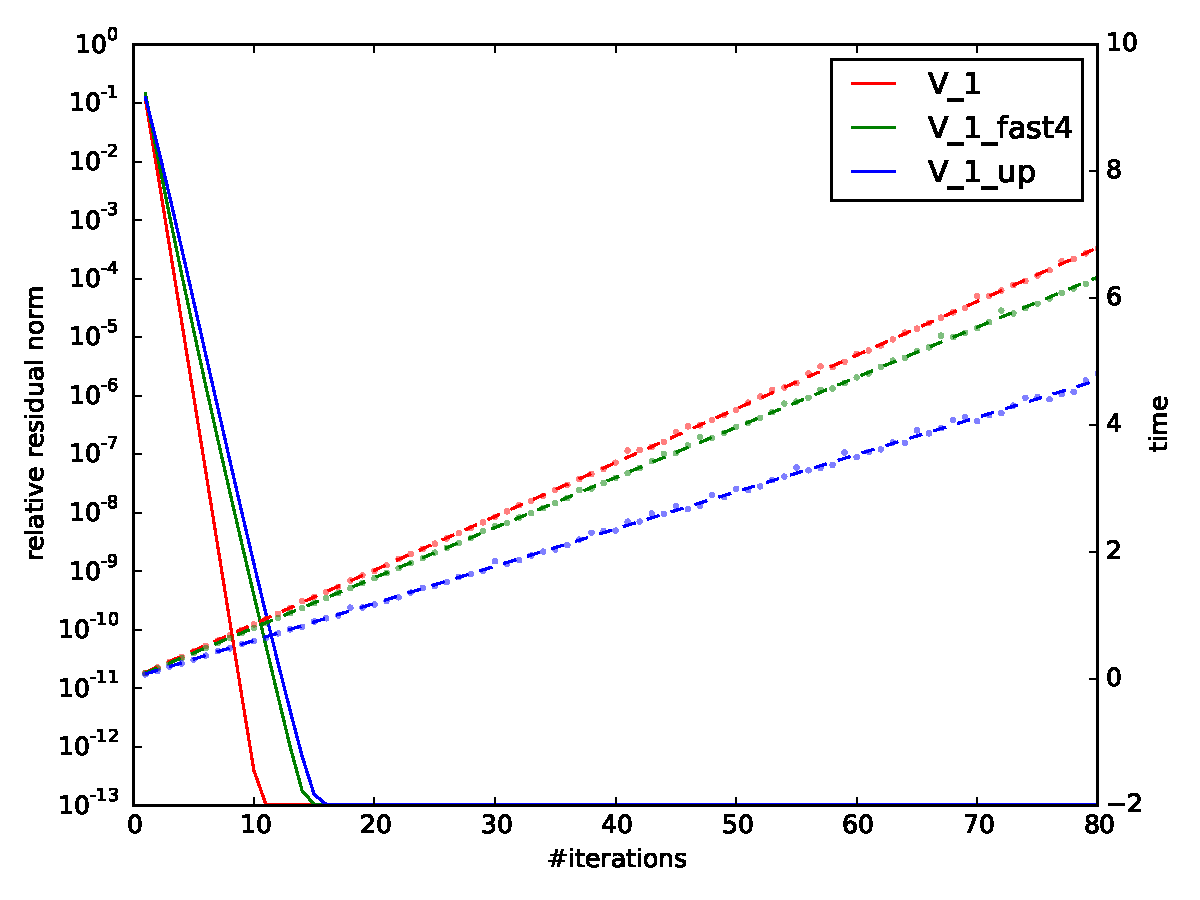
\includegraphics[width=\linewidth]{AMG2006/test/DELL/laplace/convergence_fast.pdf}
\end{frame}
\begin{frame}{Results - 80x80x80 - Laplace}
 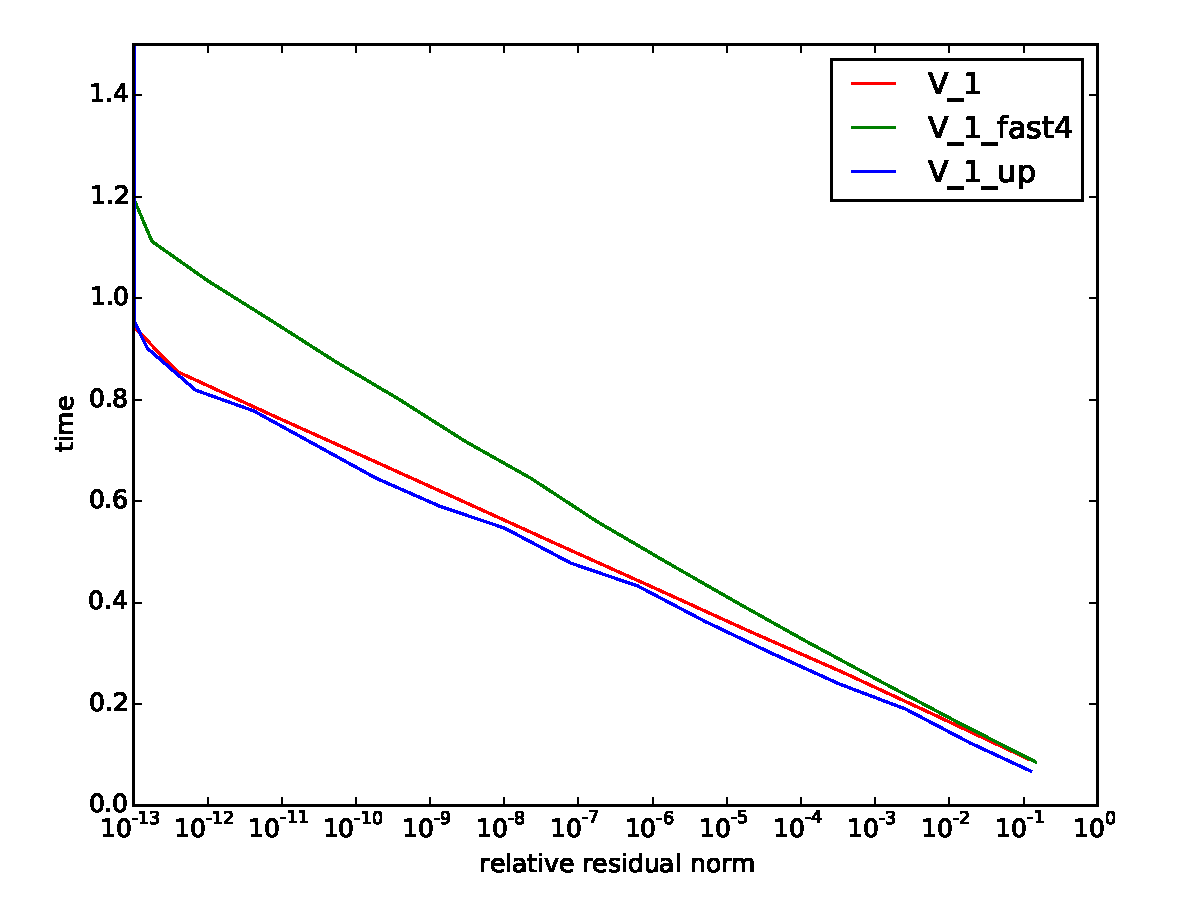
\includegraphics[width=\linewidth]{AMG2006/test/DELL/laplace/time_convergence_fast.pdf}
\end{frame}
\begin{frame}{Results - 80x80x80 - Jumps}
 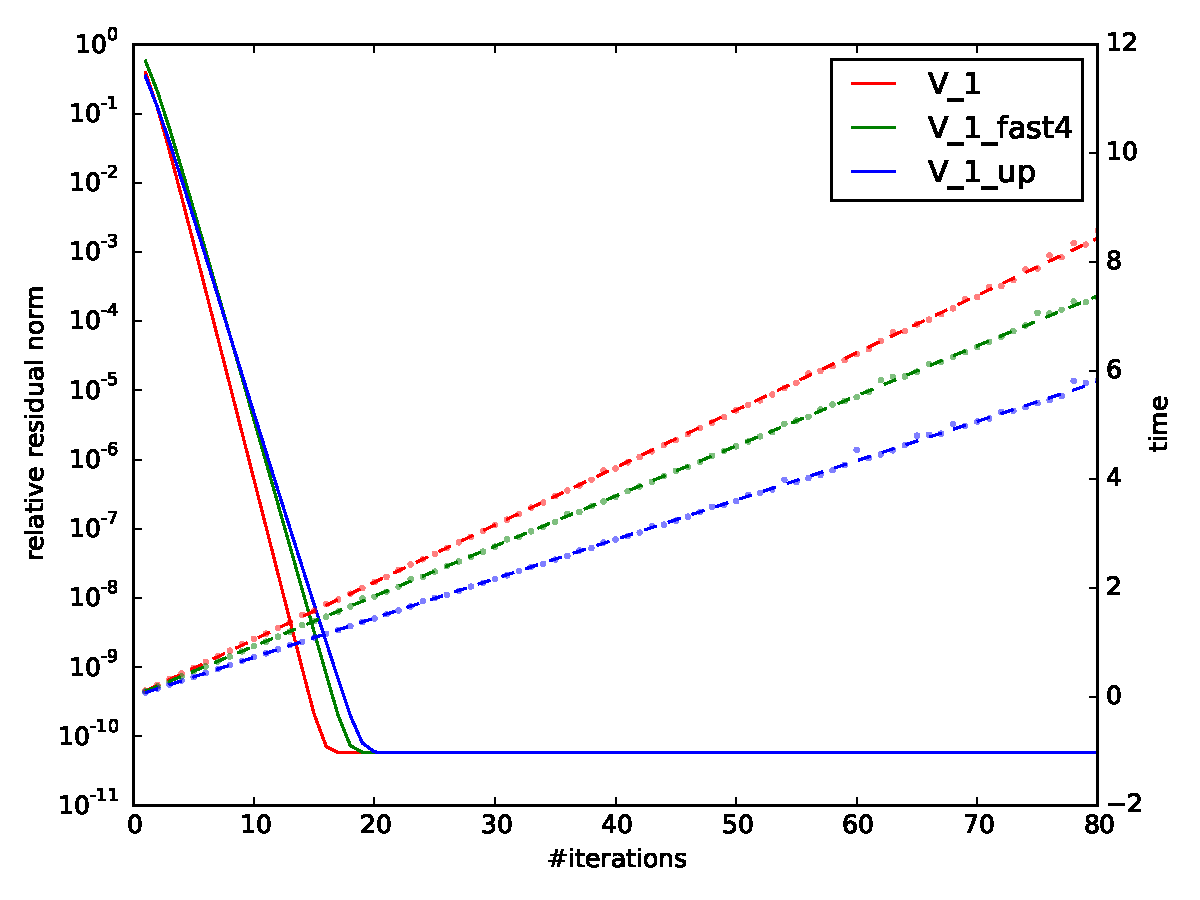
\includegraphics[width=\linewidth]{AMG2006/test/DELL/jumps/convergence_fast_10.pdf}
\end{frame}
\begin{frame}{Results - 80x80x80 - Jumps}
 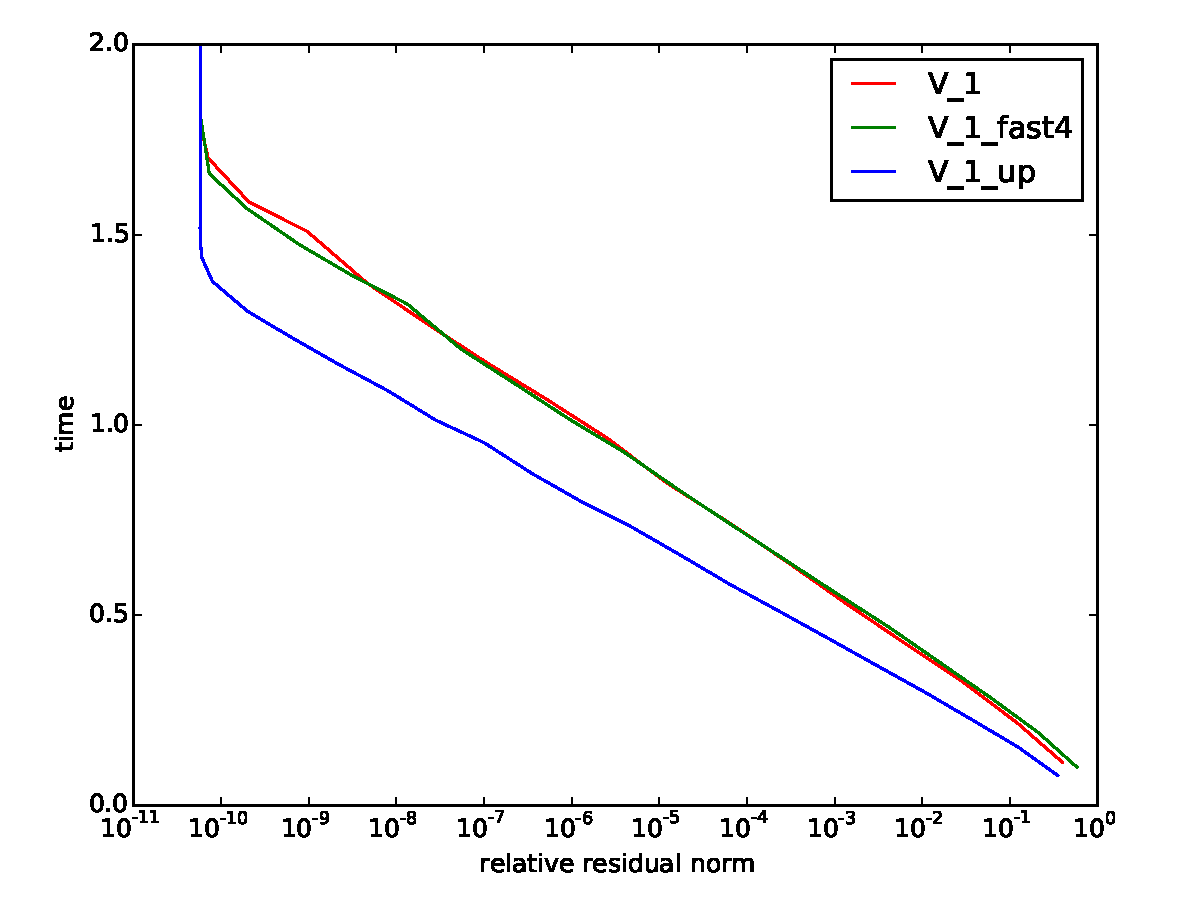
\includegraphics[width=\linewidth]{AMG2006/test/DELL/jumps/time_convergence_fast_10.pdf}
\end{frame}
\begin{frame}{Results - 40x40x40 - Jumps}
 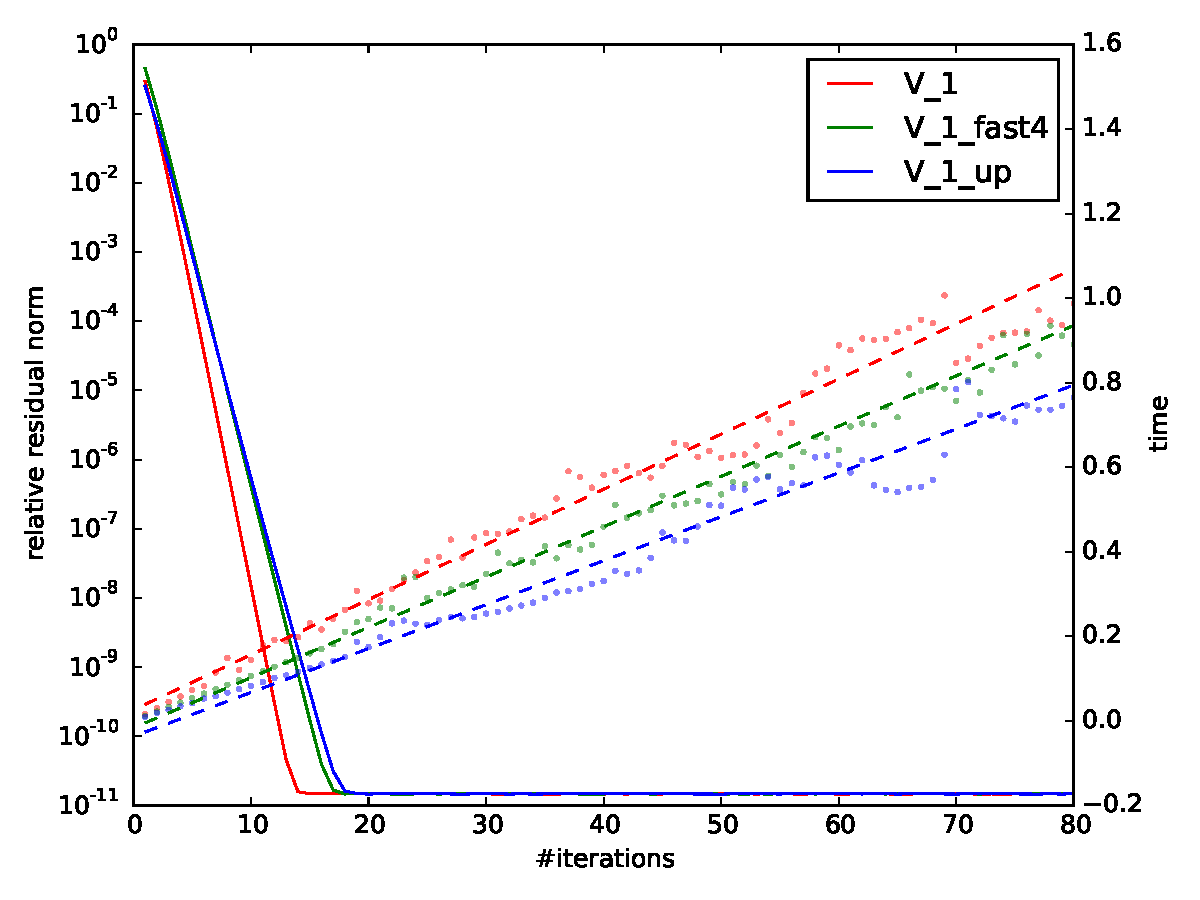
\includegraphics[width=\linewidth]{AMG2006/test/DELL/jumps/convergence_fast.pdf}
\end{frame}
\begin{frame}{Results - 40x40x40 - Jumps}
 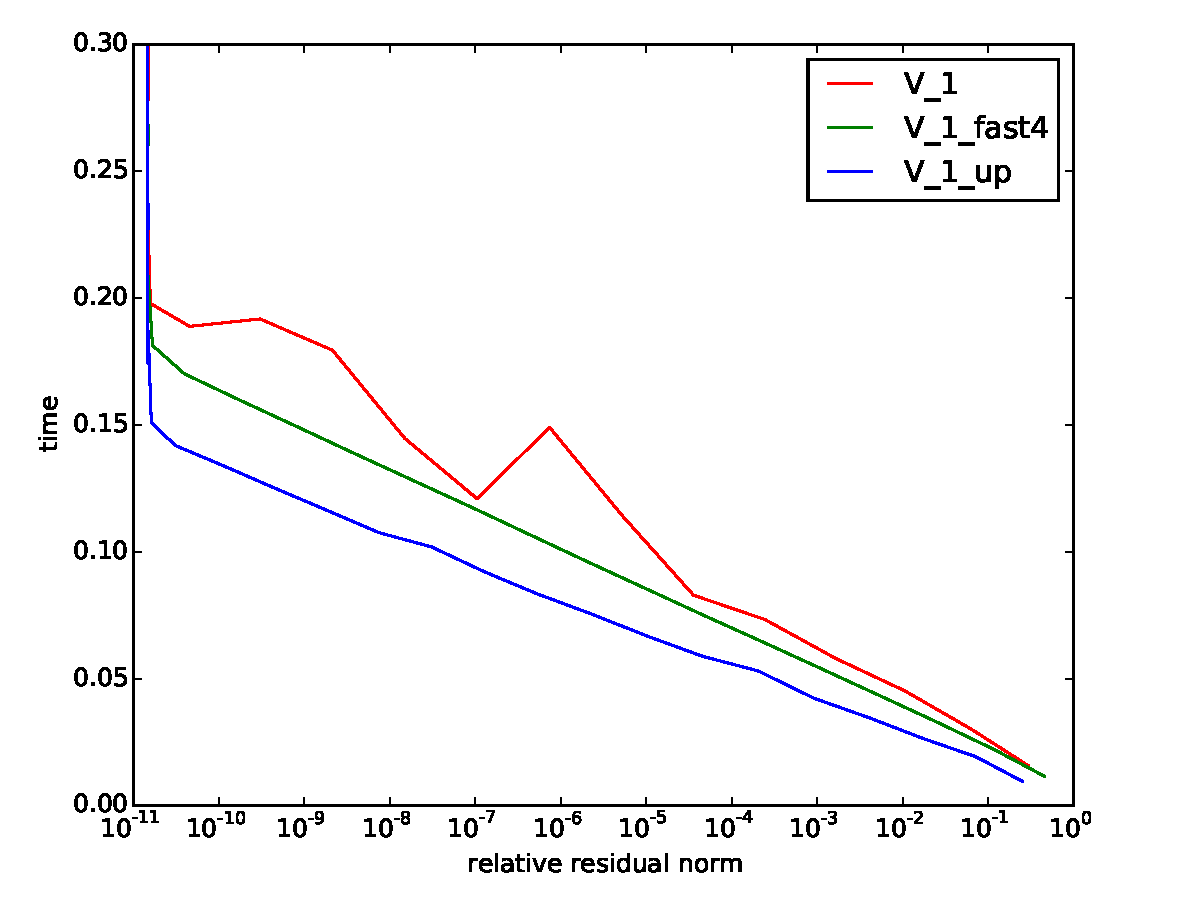
\includegraphics[width=\linewidth]{AMG2006/test/DELL/jumps/time_convergence_fast.pdf}
\end{frame}

\begin{frame}{Results on MinoTauro}
 \begin{itemize}
  \item Laplace and 27pt only
  \item Size: 180x180x180 or 240x240x240
  \item Topology: 3x3x3 or 4x4x4 or 6x6x1
 \end{itemize}
 Similar results as before. Between 1 and 30\% improvement.
 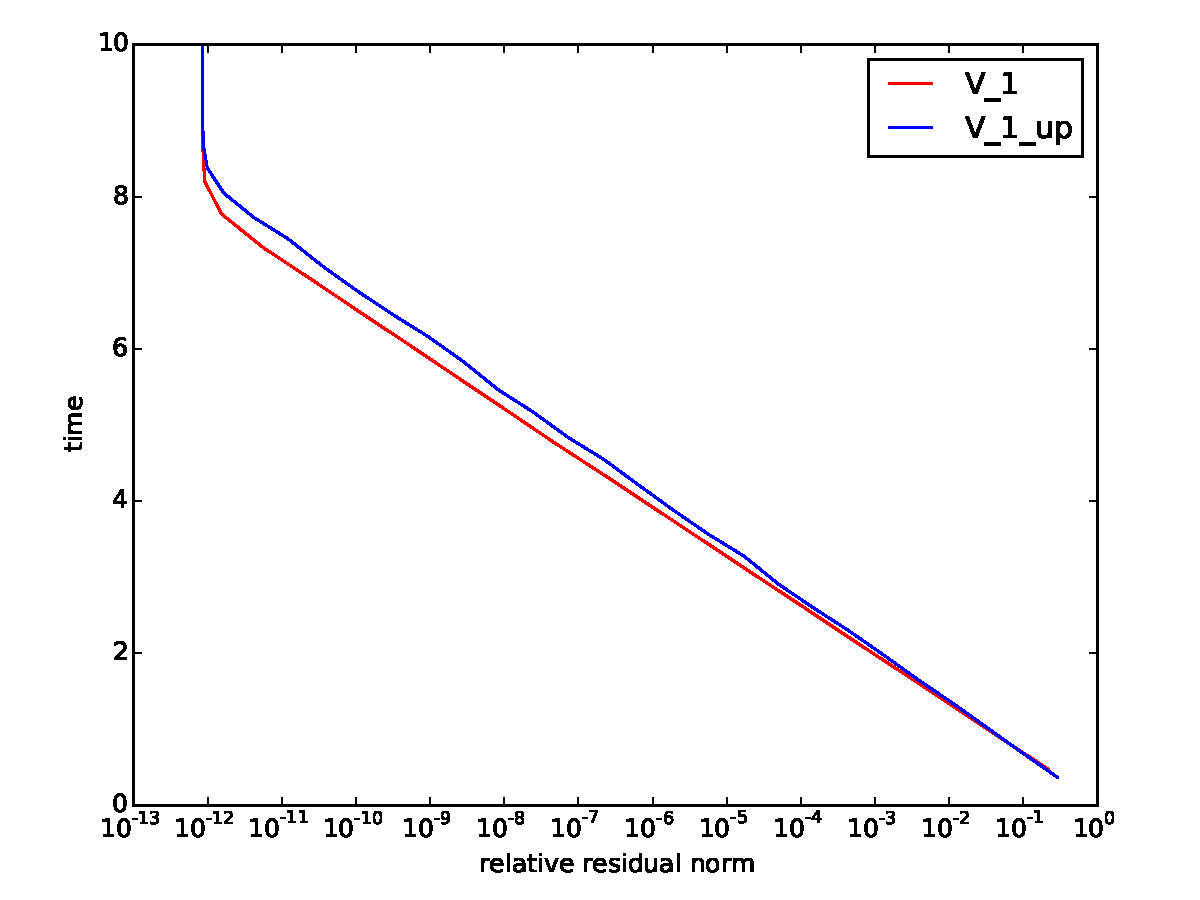
\includegraphics[width=0.33\linewidth]{AMG2006/test/MT/laplace/time_convergence_27.pdf}
 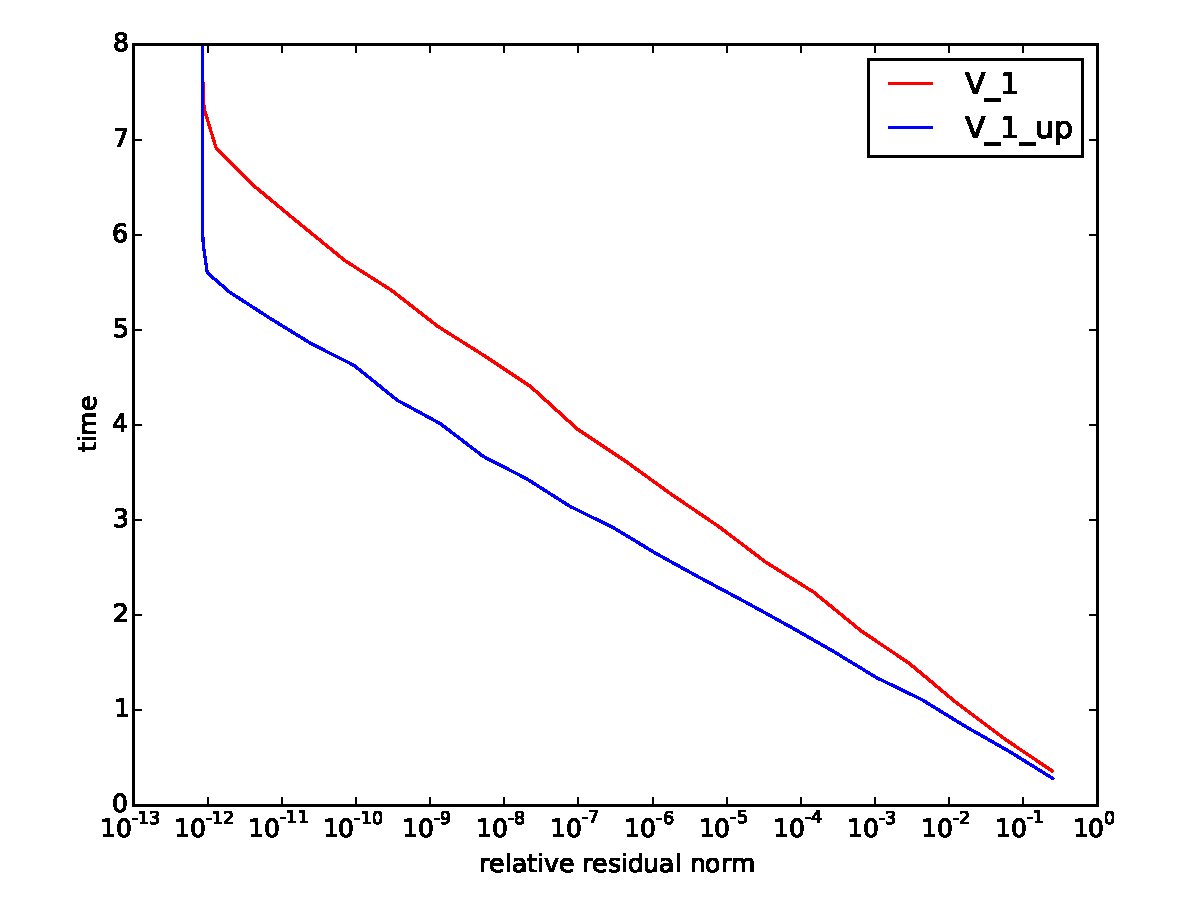
\includegraphics[width=0.33\linewidth]{AMG2006/test/MT/laplace/time_convergence_36.pdf}
 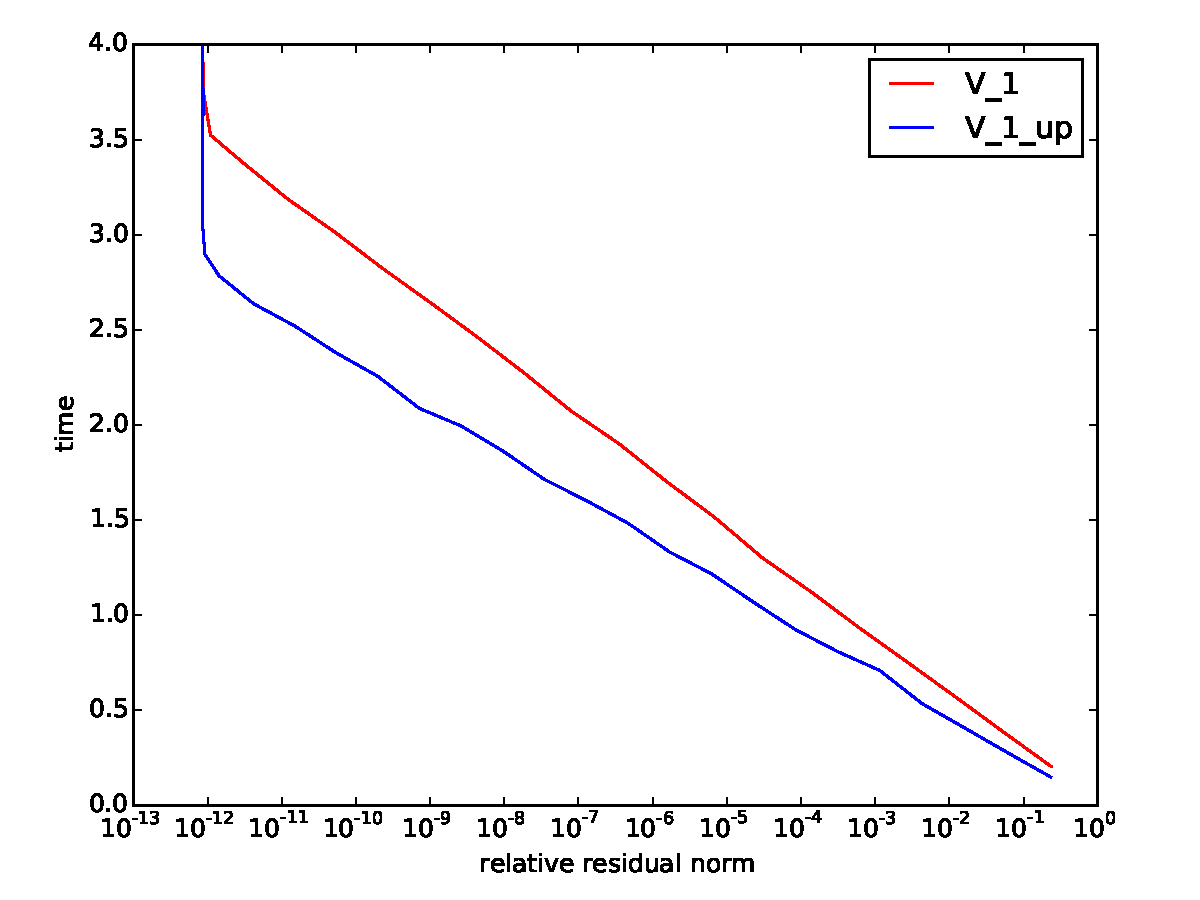
\includegraphics[width=0.33\linewidth]{AMG2006/test/MT/laplace/time_convergence_64.pdf}
\end{frame}

\begin{frame}{Relaxation function analysis}
  Only a few temporary variables, most of the variables used are the data of the input matrix.
  \begin{itemize}
    \item 2 arrays used to receive/send data
    \item 1 array used as temporary storage
    \item 2 arrays for the gaussian elimination (direct solve at last level)
    \item \textbf{3 temporary variables used as intermediate value}
    \item 5 parameters
   \end{itemize}
   MPFR version: only the single variables were changed to \texttt{mpfr\_t} type.\\
   Float version: all these aforementioned variables and arrays are changed to \texttt{float} and \texttt{float*}.
\end{frame}

\begin{frame}{Impact on execution time}
 
 The float version is longer than the original algorithm when sequential:\\
 \begin{itemize}
  \item 0.275s / 0.157s (10x10x10, 1 iteration, 1x1x1) $\rightarrow 1.75x$
  \item 2.42s / 1.36s (10x10x10, 10 iterations, 1x1x1) $\rightarrow 1.77x$
  \item 1.54s / 0.955s (10x10x10, 10 iterations, 2x1x1) $\rightarrow 1.61x$
  \item 12.25s / 7.15s (20x20x20, 10 iterations, 2x1x1) $\rightarrow 1.71x$
  \item 0.867s / 0.451s (5x5x5, 30 iterations, 1x1x1) $\rightarrow 1.92x$
  \item 4.96s / 5.00s (20x20x20, 10 iterations, \textbf{2x2x2})  $\rightarrow 0.992x$
  \item 5.29s / 5.32s (30x30x30, 10 iterations, \textbf{3x3x3})  $\rightarrow 0.994x$
  \item 0.590s / 0.606s (10x10x10, 10 iterations, \textbf{2x2x2})  $\rightarrow 0.974x$
  \item 1.020s / 1.143s (20x20x20, 10 iterations, \textbf{4x4x4})  $\rightarrow 0.89x$
 \end{itemize}
\end{frame}

\begin{frame}{Impact on execution time}
 The MPFR version adds a very big overhead compared to the original algorithm: about 50 times longer.
 \begin{tabular}{|c|c|c|c|c|}
  \hline
  \#iterations $\backslash$ \#bits & 8 & 16 & 32 & 64 \\
  \hline
  5 & 116.1 & 113.1 & 117.6 & 114.3\\
  \hline
  10 & 235.5 & 240.6 & 234.1 & 232.2\\
  \hline
  15 & 358.6 & 376.3 & 359.3 & 346.2\\
  \hline
  20 & - & 457.1 & 492.8 & 471.6 \\
  \hline
  25 & - & 587.5 & 616.6 & 614.7 \\
  \hline
  30 & - & 688.0 & 744.3 & 704.8 \\
  \hline
  35 & - & - & 904.9 & 836.9\\
  \hline
  40 & - & - & 976.2 & 950.0 \\
  \hline
  45 & - & - & - & 1012.9\\
  \hline
  50 & - & - & - & 1114.9\\
  \hline
 \end{tabular}

\end{frame}

\begin{frame}{Impact on accuracy}
  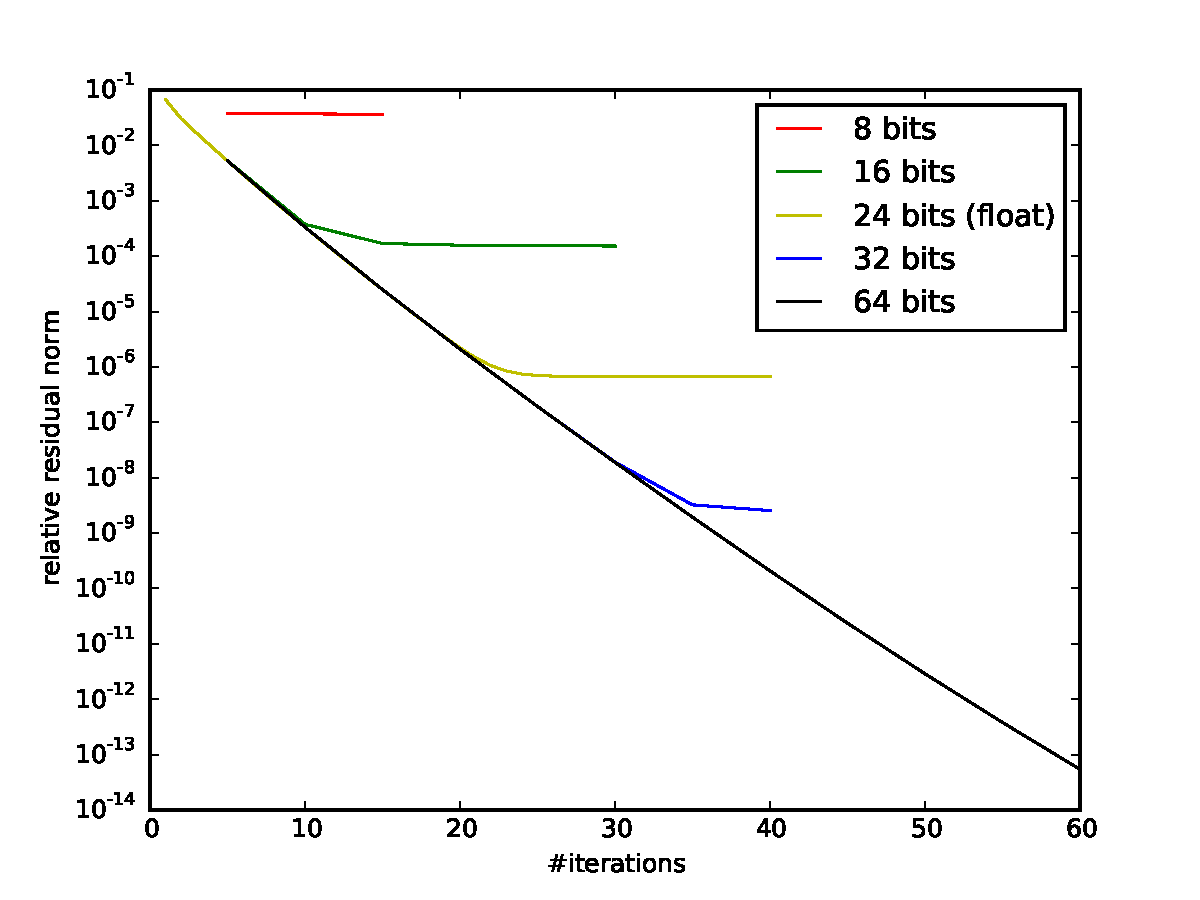
\includegraphics[width=\linewidth]{AMG2006/test/MPFR/bits_convergence.pdf}
\end{frame}

\begin{frame}[fragile]{Impact on accuracy}
  $\Rightarrow$ \texttt{res}, \texttt{res0} and \texttt{res2} variables define the accuracy of the relaxation step and the accuracy of the whole algorithm.
  \resizebox{0.8\linewidth}{!}{\lstinputlisting[language=C, firstline=1832, lastline=1848]{AMG2006/parcsr_ls/par_relax.c}}
\end{frame}



\end{document}
